% Created 2021-10-06 mar 13:05
% Intended LaTeX compiler: pdflatex
%%% Local Variables:
%%% LaTeX-command: "pdflatex --shell-escape"
%%% End:
\documentclass[11pt]{article}
\usepackage[utf8]{inputenc}
\usepackage[T1]{fontenc}
\usepackage{graphicx}
\usepackage{grffile}
\usepackage{upgreek}
\usepackage{longtable}
\usepackage{wrapfig}
\usepackage{rotating}
\usepackage[normalem]{ulem}
\usepackage{amsmath}
\usepackage{textcomp}
\usepackage{amssymb}
\usepackage{listings}
\usepackage{capt-of}
\usepackage{hyperref}
\hypersetup{colorlinks=true, linkcolor=black}
\setlength{\parindent}{0in}
\usepackage[margin=1.1in]{geometry}
\usepackage[spanish]{babel}
\usepackage{mathtools}
\usepackage{palatino}
\usepackage{fancyhdr}
\usepackage{sectsty}
\usepackage{engord}
\usepackage{cite}
\usepackage{graphicx}
\usepackage{setspace}
\usepackage[compact]{titlesec}
\usepackage[center]{caption}
\usepackage{placeins}
\usepackage{tikz}
\usetikzlibrary{positioning}
\usetikzlibrary{bayesnet}
\usetikzlibrary{shapes.geometric}
\usetikzlibrary{decorations.text}
\usepackage{color}
\usepackage{amsmath}
\usepackage{minted}
\usepackage{pdfpages}

\newcommand*{\B}{\mathbb{B}}
\newcommand*{\C}{\mathbb{C}}
\newcommand*{\R}{\mathbb{R}}
\newcommand*{\ra}{\rangle}
\newcommand*{\la}{\langle}

\def\inline{\lstinline[basicstyle=\ttfamily,keywordstyle={}]}

\titlespacing*{\subsection}{0pt}{5.5ex}{3.3ex}
\titlespacing*{\section}{0pt}{5.5ex}{1ex}
\author{José Antonio Álvarez Ocete\\ Francisco Javier Sáez Maldonado}
\date{\today}
\title{D-Wave: computación cuántica mediante \emph{quantum annealing}\\\medskip
\large Procesamiento de Datos a Gran Escala - Práctica opcional}

\begin{document}

\maketitle

\tableofcontents

\section{Motivación y objetivos}

En esta asignatura hemos expuesto las bases teóricas de la computación cuántica desde el álgebra lineal y la teoría de la computación, para posteriormente explicar los algoritmos más destacados de este nuevo paradigma, como la teleportación cuántica o el algoritmo de Shor. \\

En esta práctica opcional exploraremos otra forma de implementar computación cuántica, basándonos en evolución adiabática y \emph{quantum annealing} (usualmente mal traducido como \emph{enfriamiento cuántico}). En particular exploraremos los siguientes temas:

\begin{itemize}
	\item El \emph{quantum annealing} comparte algunas de las bases con la computación cuántica basada en circuitos, describiremos de forma superficial e intuitiva \textbf{las bases de la mecánica cuántica} que subyacen a ambos modelos y describiremos dónde residen las diferencias entre ambos.
	
	\item Explicaremos en profundidad \textbf{óomo funcionan los ordenadores D-Wave}, así como los problemas de optimización que pueden resolver.

	\item Comentaremos en detalle \textbf{el problema de ensamblaje del genoma}, y cómo resolverlo utilizando ordenadores D-Wave.
	
	\item Veremos los resultados obtenidos los computadores \emph{D-Wave 2000} y \emph{Advantage} al resolver este problema particular.
\end{itemize}

Este problema esta basado en el Trabajo Fin de Grado de uno de los componentes de esta pareja de prácticas, José Antonio Álvarez. Dicho documento puede encontrarse en \href{https://github.com/Ocete/TFG/blob/main/thesis.pdf}{el respectivo repositorio de GitHub}.

\section{Desarrollo}

\subsection{El modelo de la mecánica cuántica}

Realizaremos una descripción superficial sobre la gran base teórica existente en este respecto. Para más detalle, consúltese el TFG al completo. \\

La mecánica cuántica esta basado en cuatro ``simples'' postulados, sobre los que se construye toda la teoría necesaria para la física cuántica y la computación cuántica en particular. Los enunciamos y explicamos a continuación.

\begin{enumerate}
	\item El primer postulado nos indica \textbf{cómo describir matemáticamente un sistema físico}: \emph{Cualquier sistema físico aislado tiene asociado un espacio de Hilbert llamado el \textbf{espacio de estados}. El estado del sistema queda totalmente descrito por un vector unitario de dicho espacio, y se denomina \textbf{vector estado}.} \\
	
	Dado que todo espacio de Hilbert finito es isomorfo a $\mathbb C^n$, donde $n$ es la dimensión de dicho espacio, los vectores estados serán vectores unitarios de $\C^n$ para cierto $n$. En particular, un \emph{qubit} se define como un vector estado del espacio de estados $\C^2$. Es decir, un vector unitario de $\C^2$:
	
	\[ |\varphi\ra = \alpha|0\ra + \beta|1\ra \]
	
	Donde $|\alpha|, |\beta| = 1$.
	
	\item El segundo postulado nos indica \textbf{cómo medir nuestro sistema} en este paradigma. De igual forma que medimos la velocidad de un coche o la altura de una persona, hemos de ser capaces de medir ciertas variables en este sistema. El enunciado formal implica unos operadores de medida que únicamente complicarían este texto, así que nos ceñimos a las implicaciones del mismo. \\
	
	La consecuencia más relevante es que \textbf{al medir un sistema, lo alteramos}. Esto se traduce en la computación cuántica en el colapso de los qubits tras la medida a uno de los estados. Adicionalmente, esto establece uno de los principales inconvenientes de la computación cúantica: la imposibilidad de conocer exactamente las amplitudes de un estado, lo que desembocará en el \textbf{Teorema de no clonación}.
	
	\item El tercer postulado es el más relevante para nosotros pues \textbf{crea la distinción entre el modelo de computación cuántica basado en circuitos y el basado en \emph{quantum annealing}}. \textbf{Describe la evolución del sistema} y tiene dos enunciados equivalentes que provocan la distinción mencionada. \\
	
	En su primera forma, el postulado dicta que la evolución de un sistema cuántico cerrado queda descrita por una \textbf{transformación unitaria} que unicamente depende de los tiempos $t_1,t_2$ en los que se compara el sistema:
	
	\[ |\varphi_{t_2}\ra = U|\varphi_{t_1}\ra \]
	
	En el modelo de circuitos de la computación cuántica este postulado establece las bases teóricas de las puertas cúanticas: transformaciones unitarias aplicadas al estado del sistema (qubits). \\
	
	La segunda forma de este postulado viene de la mano de la ecuación de Schrödinger, la cual exploraremos en detalle más adelante.
	
	\item Finalmente, el cuarto postulado nos habla de \textbf{la composición de sistemas cuánticos}. Dicta lo siguiente: \emph{El espacio de estados de un sistema físico compuesto es el \textbf{producto tensorial} de los espacios de estados de los subsistemas. Además, el vector de estado del sistema es el producto tensorial de los vectores de estado de los subsistemas:} $|\varphi_1\ra \otimes \dotsc \otimes |\varphi_n\ra$.
	
	La diferencia más relevante en nuestro caso entre el producto vectorial al que estamos acostumbrados y el producto tensorial es que la dimensión de los espacio se multiplica en vez de sumarse: $\R^2 \times \R^3 = \R^5$ mientras que $\R^2 \otimes \R^3 = \R^6$. Es por ello que al añadir qubits a nuestro sistema, la información crece de manera exponencial y no lineal como ocurre en el caso de los bits. \\
	
	Como corolario inmediato de este postulado obtenemos que un sistema de $n$ qubits tiene por espacio de estados asociado $\C^{2^n}$. 
\end{enumerate}

\subsection{Quantum annealing y evolución adiabática}

Como se menciono anteriormente, Schrödinger proporcionó una versión equivalente de este postulado. Esta dicta que la evolución temporal de nuestro sistema viene dada por la famosa \textbf{ecuación de Schrödinger}:

\[ i \hbar \frac{d|\varphi\ra}{dt} = H|\varphi\ra \]

Donde $\hbar$ es la constante de Plank, $i$ es la unidad imaginaria y $H$ es un operador hamiltoniano. Aunque esta ecuación es intimidante, es más sencilla de lo que parece. Puesto que $\hbar$ e $i$ son constantes, lo único desconocido es el operador $H$ (una matriz). Con ello conocemos la derivada del vector de estados. Esto es, cómo evoluciona con el tiempo. \\

La idea que reside bajo el \emph{quantum annealing} es elegir nosotros el hamiltoniano del sistema para hacer que evolucione a nuestro antojo. Utilizaremos la descomposición singular del hamiltoniano:

\[ H = \sum_E E |v_E\ra\la v_E| \]

Donde $E$ son los valores propios de $H$ y $v_E$ los respectivos vectores propios. A los valores propios se les suele denominar \emph{energías}, ya que describen la energía del estado propio asociado. Al estado propio con menor energía se le denomina \emph{estado base} o \emph{ground state}. \\

En particular, utilizaremos un hamiltoniano que variaremos con el tiempo:

\[ H(t) = \sum_{E(t)} E(t) |v_{E(t)}\ra\la v_{E(t)}| \quad t \in [t_{initial}, t_{final}] \]

Aqui nos apoyamos del \textbf{Teorema de Evolución Adiabática}: un sistema físico se mantiene en un estado propios si las alteraciones realizadas al sistema se producen lo suficientemente despacio y hay un \emph{hueco} lo suficientemente grande entre el valor propio asociado y el resto de valores propios. \\

En primer lugar, demos una visión intuitiva de este teorema. Supongamos que tenemos un péndulo simple oscilando sujeto en su punto superior con la mano. Si movemos la mano muy despacio, la perturbación que sufre el péndulo es inócua, y este permanecerá en su estado propio. Sin embargo, si movémos rápidamente la mano, el péndulo variará drásticamente su trayectoria. \\

Para nuestro caso, buscaremos que el hamiltoniano varíe entre dos valores constantes: $H_{initial}$ y $H_{final}$:

\[ H(s) = A(s) \cdot H_{initial} + B(s) \cdot H_{final} \quad \forall s \in [t_{initial}, t_{final}] \]

Donde $A(s)$ disminuirá con el tiempo y $B(s)$ aumentará.

\begin{figure}[H]
	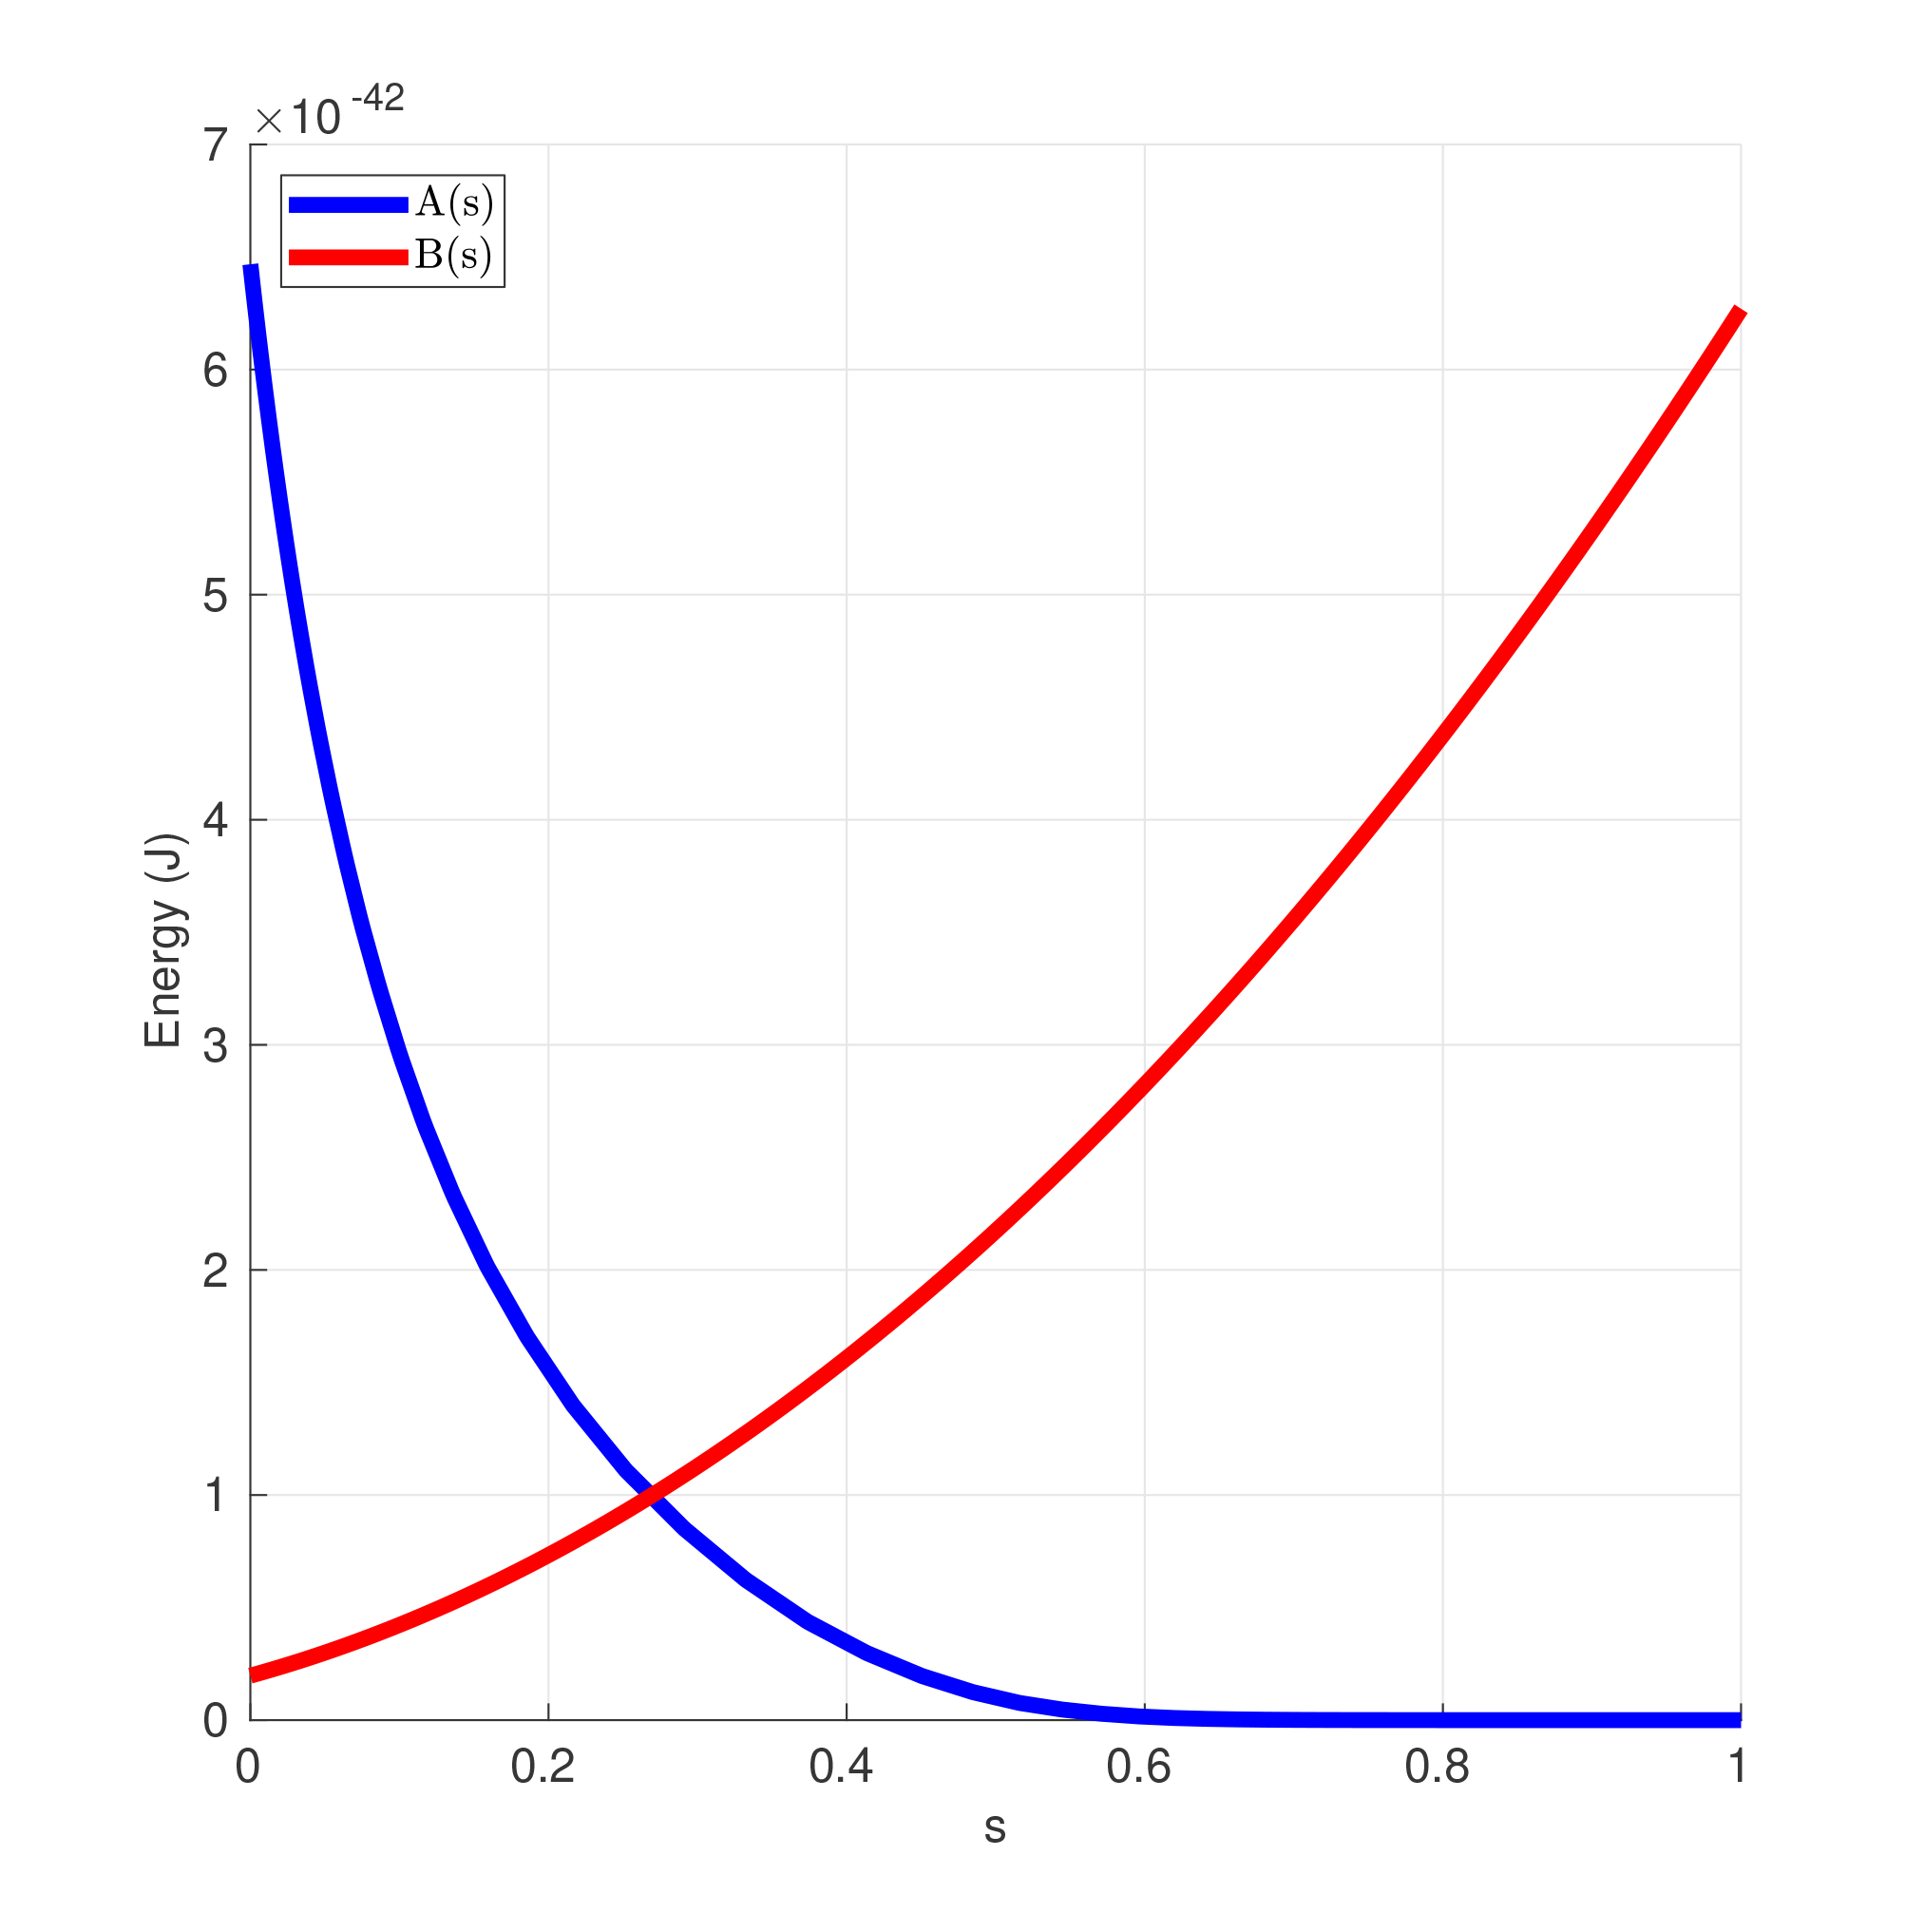
\includegraphics[scale=.14]{figures/dwave-annealing-functions}
	\centering
	\caption{Funciones de \emph{Annealing} utilizadas en los sistemas D-Wave 2X}\
\end{figure}

La codificación inicial, $H_{initial}$, será muy sencilla. De esta forma podremos conocer nuestro sistema a la perfección. De hecho, nuestro estado inicial del sistema será el estado base de $H_{initial}$. Si se cumple el teorema de evolución adiabática (volveremos ahora para ver cuando ocurre), tras la evolución nuestro sistema estará en el estado base de $H_{final}$. \\

Dado un problema de optimización, codificaremos $H_{final}$ para que el estado propio de menor energía sea el mínimo de nuestra función objetivo. De esta forma, tras aplicar evolución adiabática obtendremos el estado base. Esto es, la solución que minimiza nuestra función objetivo. \\

La ecuación final utilizada en la práctica por los sistemas D'Wave es la siguiente:

\[ H(s) = \underbrace{- \frac{A(s)}{2} \bigg( \sum_i \upsigma_x^{(i)} \bigg)}_\text{Initial Hamiltonian} 
+ \underbrace{\frac{B(s)}{2} \bigg( \sum_i h_i \upsigma_z^{(i)} + \sum_ {i > j} J_{i,j} \upsigma_z^{(i)} \upsigma_z^{(j)} \bigg)}_\text{Final Hamiltonian} \]

Tras esta explicación quedan dos cuestiones por resolver. En primer lugar, ¿Qué es el ``hueco'' de la segunda hipótesis del teorema de evolución adiabática y cuándo se cumple? Este hueco hace referencia a la distancia entre los valores propios. Durante la evolución temporal que se produce en el sistema, los valores propios también varían. Cuanto más se acerquen dichos valores, más probable es que el sistema ``salte''  a otro de los estados propios del sistema. Este fenómeno se conoce como \emph{quantum tunneling}.

\begin{figure}[H]
	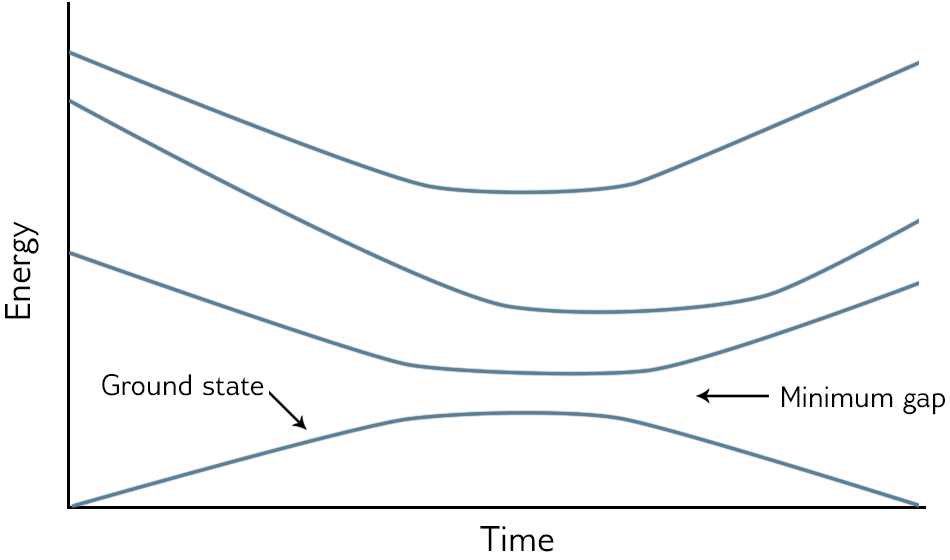
\includegraphics[scale=.3]{figures/dwave-eigenspectrum.png}
	\centering
	\caption{Ejemplo de evolución temporal de valores propios}
	\label{fig:dwave-eigenspectrum}
\end{figure}

Dado un problema arbitrario es difícil conocer la evolución de los valores propios temporalmente y mucho menos controlarla. Sin embargo, si la evolución es lo suficientemente lenta, podemos disminuir la probabilidad de dicho salto. Ejecutando el algoritmo en múltiples ocasiones -esto es, utilizando métodos de Monte Carlo- aumentaremos la posibilidad de obtener la solución óptima. Aún así, soluciones cercanas al estado base también obtendrán bajos valores de la función objetivo. \\

Por otro lado, resta preguntarse qué problemas podemos codificar en un hamiltoniano y cómo hacerlo. Esto serán los problemas QUBO.

\subsection{Los problemas QUBO}

Los modelos QUBO e Ising pueden codificarse de forma sencilla en un hamiltoniano. En este texto nos centramos en el primero por brevedad, pero el segundo es equivalente. En la práctica, problemas que no son de optimización se transforman en problemas de optimización y posteriormente se codifican como problemas QUBO para ser resueltos utilizando \emph{quantum annealing}. Estudiámos a continuación los problemas QUBO y codificar otros problemas en este formato. \\

Sea $\B = \{0,1\}$ y $f_Q: \B^n \longrightarrow \R $ una función polinómica cuadrática sobre variables binaria:

\[ f_Q(x) = \sum_{i=1}^n \sum_{j=1}^i q_{ij} x_i x_j \]

donde $x_i \in \B$ para $i \in \{1, \cdots, n\}$ y los coeficientes $q_{ij} \in \R$ para $1 \leq j \leq i \leq n$. Un problema binario de optimización sin restricciones (\textbf{\emph{quadratic unconstrained binary optimization} o QUBO}) consiste en encontrar el vector binario $x'$ que minimiza $f_Q$:

\[ x' = \underset {x \in \B^n }{\arg \min} ~ f_Q(x) \]

La ventaja de los problemas QUBO es que tienen una descripción matricial sencilla:

\[ f_Q(x) = x^T Q x \]

donde $Q$ es una matriz $n \times n$ simétrica que contiene los coeficientes $q_{ii}$ en su diagonal y $q_{ij} / 2$ en la posición $(i,j)$ si $i \neq j$. \textbf{Esta matriz $Q$ será nuestro hamiltoniano $H$}. ¿Qué problemas pueden ser codificados de esta forma? A través de una serie de transformaciones sencillas, todo problema cuadrático con restricciones lineales puede ser transformado a un problema de minimización sin restricciones, incluyendo las restricciones del problema original como penalizaciones en nuestra función de pérdida. \\

En el texto original queda explicado el método de transformación general, así como algunos de los problemas NP-duros más famosos: el problema de corte máximo (Max-Cut), Max SAT-2, el coloreado de grafo y el viajante de comercio. \\

Este último es especialmente relevante para su posterior aplicación en el problema del ensamblaje del genoma. En dicho problema, dado un grafo $G$ con nodos $v_1, \ldots, v_n$, y con pesos asociados a cada lado del grafo $w_{i,j}$ para todo $i,j \in [1, \ldots, n]$, buscamos un camino hamiltoniano (que pasa por todos los nodos del grafo una única vez) con pesos mínimos. \\

Para ello definimos $n^2$ variables binarias $x_{i,j}$, que valdrán $1$ si y sólamente si nuestro camino pasa por el nodo $i$ en el instante $j$. Hemos de añadir una serie de restricciones adicionales para que se cumplan las condiciones de ser un camino hamiltoniano por el grafo: unicamente pasamos por un nodo en el instante $j$, y nunca pasamos dos veces por el mismo nodo. A estas condiciones las denominamos \text{colocación} y \textbf{repetición} respectivamente. \\

Añadimos adicionalmente unos pesos negativos en la diagonal de la matriz para, si hiciese falta, premiar el que se asignen nodos. Denominamos a esta condición extra \textbf{(self-bias)}. Nuestra función de pérdida final, sin restricciones, es la siguiente:

\begin{equation}
	\begin{alignedat}{3}
		& \text{Minimize }	&& \sum_{i=0}^{n-1} \sum_{j=0}^{n-1} w_{i,j}\sum_{p=0}^{n-1} x_{i,p}x_{j,p+1} & \\
		& && + a \sum_{i=0}^{n-1} \sum_{p=0}^{n-1} x_{i,p} & \qquad \text{(self-bias)} \\
		& && + b \sum_{i=0}^{n-1} \Big( \sum_{p=0}^{n-1} x_{i,p} - 1 \Big)^2 & \qquad \text{(repetición)} \\
		& && + c \sum_{p=0}^{n-1} \Big( \sum_{i=0}^{n-1} x_{i,p} - 1 \Big)^2 & \qquad \text{(colocación)}
	\end{alignedat}
\end{equation}

Donde $a,b,c$ son tres parámetros reales que codifican el peso dado a cada restricción. Hemos transformado nuestro problema original con un grafo de $n$ nodos en un problema QUBO con $n^2$ variables. Veámos un ejemplo de esta transformación. Dado el siguiente grafo:

\begin{figure}[H]
	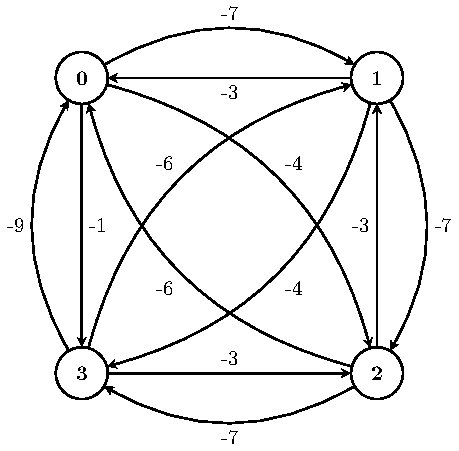
\includegraphics[scale=1.1]{figures/salesman-example.pdf}
	\centering
	\label{fig:salesman-example}
\end{figure}

Dado que el grafo tiene $4$ nodos, definimos $4^2 = 16$ variables binarias y las renombramos:

\[ (x_{0,0}, x_{0,1}, x_{0,2}, x_{0,3}, x_{1,0}, x_{1,1}, x_{1,2}, \dots, x_{3,2}, x_{3,3}) =
(x_1, x_2, x_3, x_4, x_5, x_6, x_7, \dots, x_{15}, x_{16}) \]

Utilizando los valores $a = 0$ y $b = c = 13$ para los parámetros podemos obtener la expresión de la función de pérdida para nuestro problema, que podemos expresar en forma matricial con la expresión 

\[ f_Q(x) = x^T Q x. \]

\begin{figure}[H]
	\makebox[\textwidth][c]{
		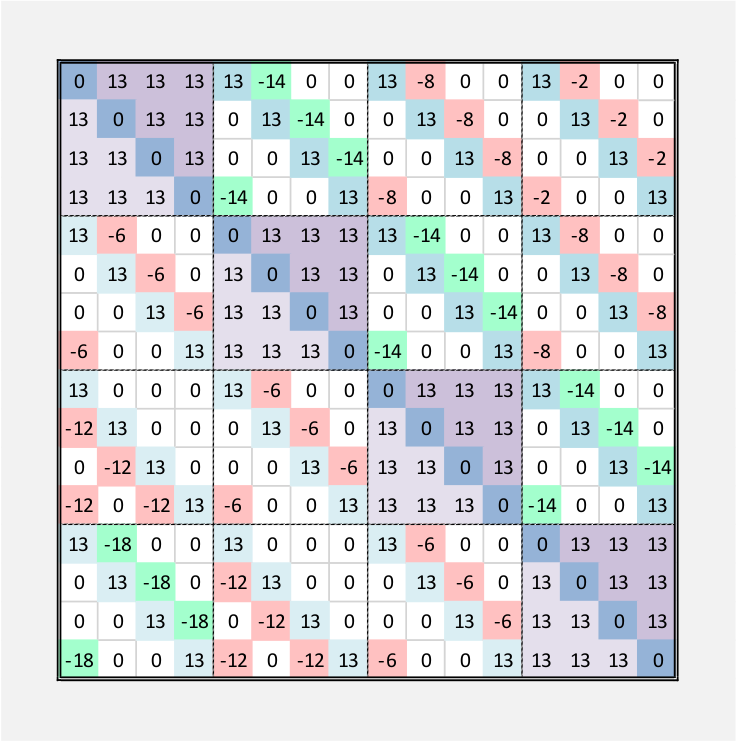
\includegraphics[scale=0.4]{figures/salesman-Q-matrix.png}
	}
	\centering
	\caption{Matriz Q final}
\end{figure}

Esta matriz cuadrada puede verse como una matriz de adyacencia de un grafo con 16 de nodos para obtener una visión intuitiva de las restricciones:

\begin{table}[H]
	\centering
	\makebox[\textwidth][c]{
		\begin{tabular}{ccc}		
			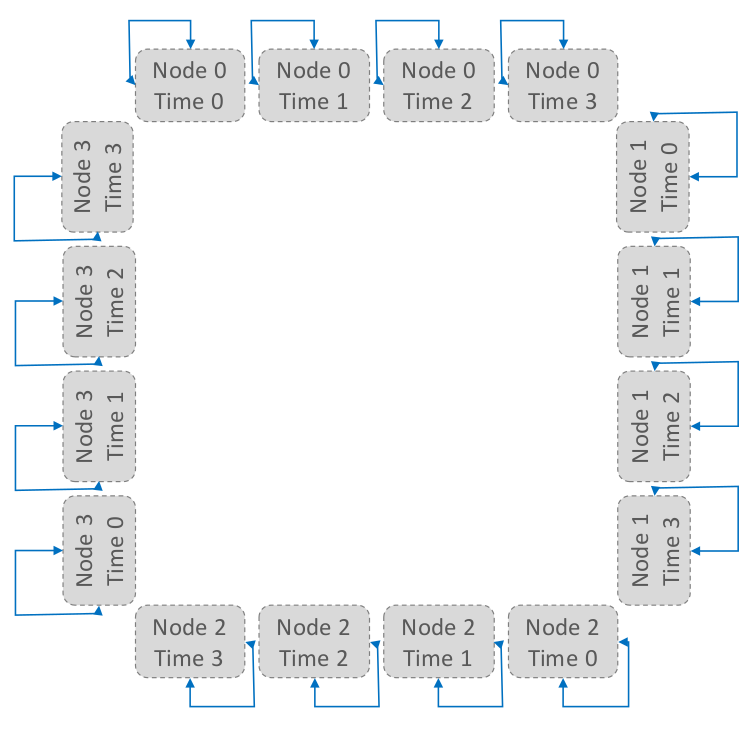
\includegraphics[scale=0.2]{figures/salesman-penalties1.png} &
			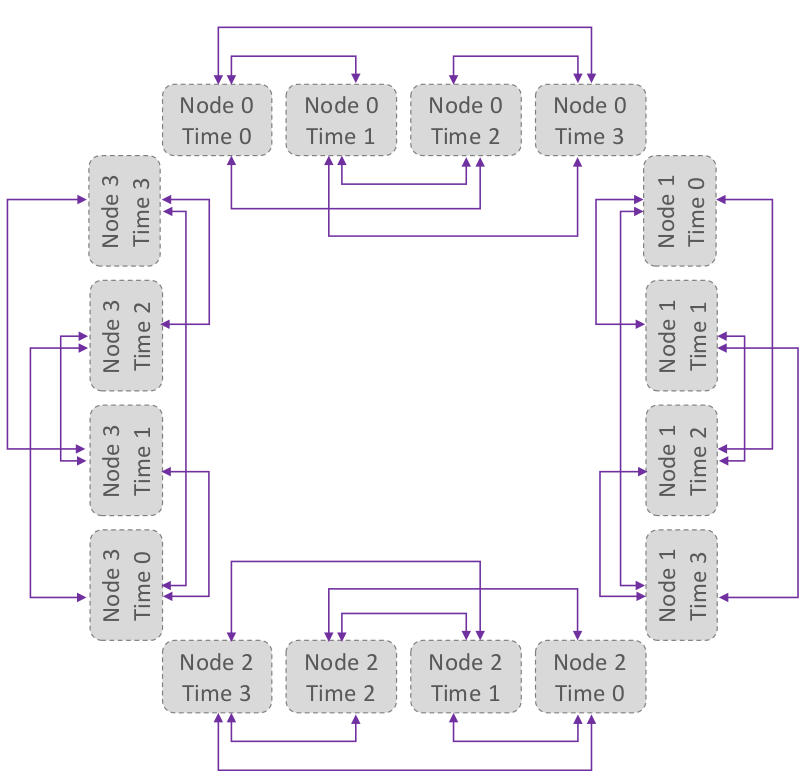
\includegraphics[scale=0.2]{figures/salesman-penalties2.png} &
			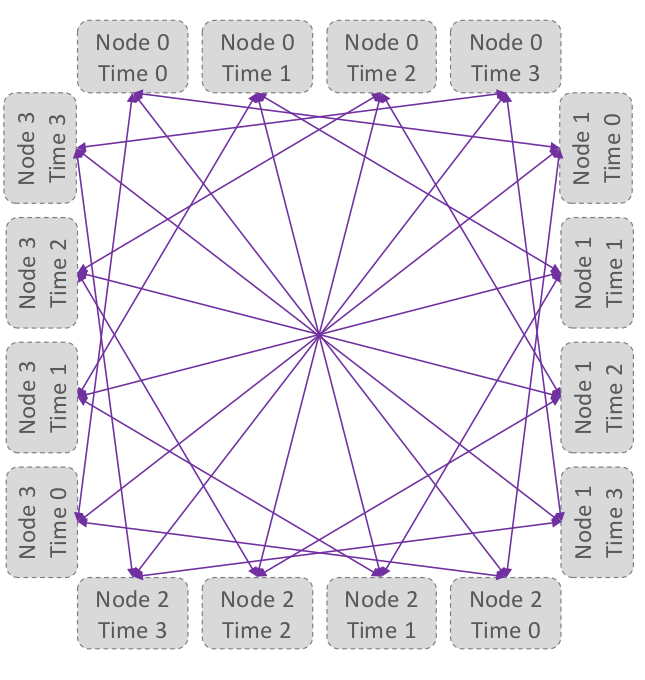
\includegraphics[scale=0.2]{figures/salesman-penalties3.png} \\
			
			1: Self-bias & 2: Repetición & 3: Colocación \\
			
			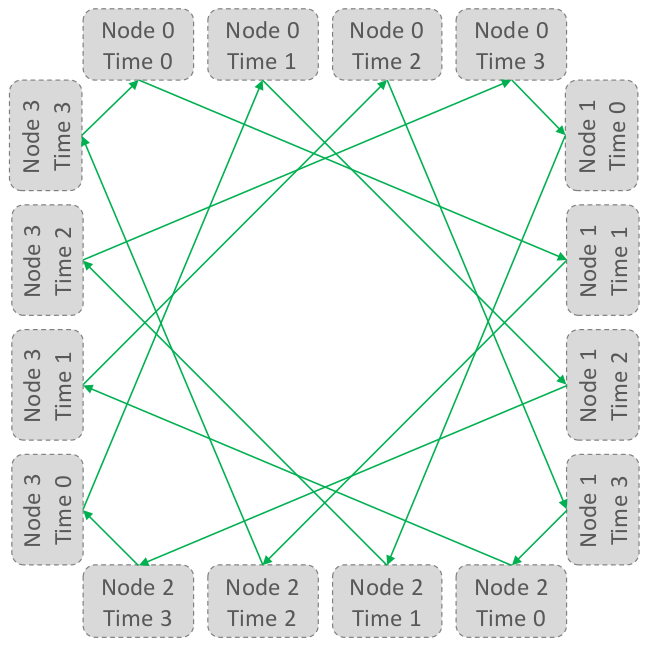
\includegraphics[scale=0.2]{figures/salesman-penalties4.png} &
			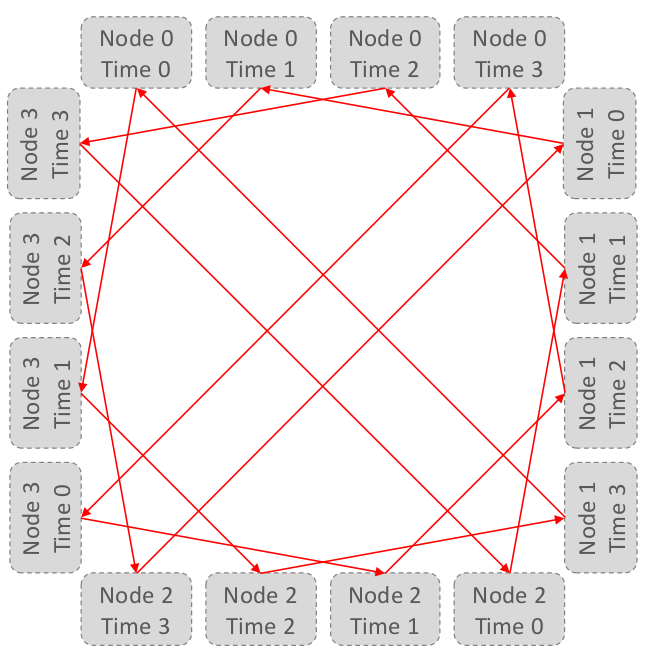
\includegraphics[scale=0.2]{figures/salesman-penalties5.png} &
			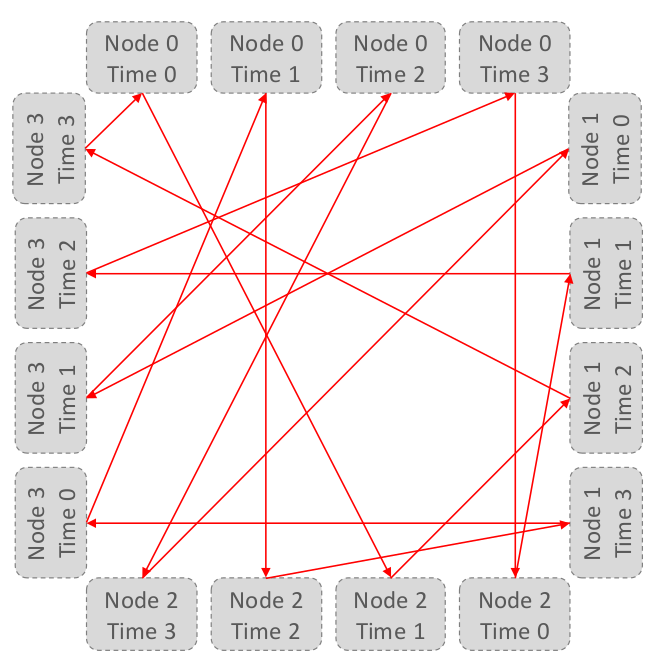
\includegraphics[scale=0.2]{figures/salesman-penalties6.png} \\
			
			4: Type A tours & 5: Type B tours & 6: Type C tours \\
			
			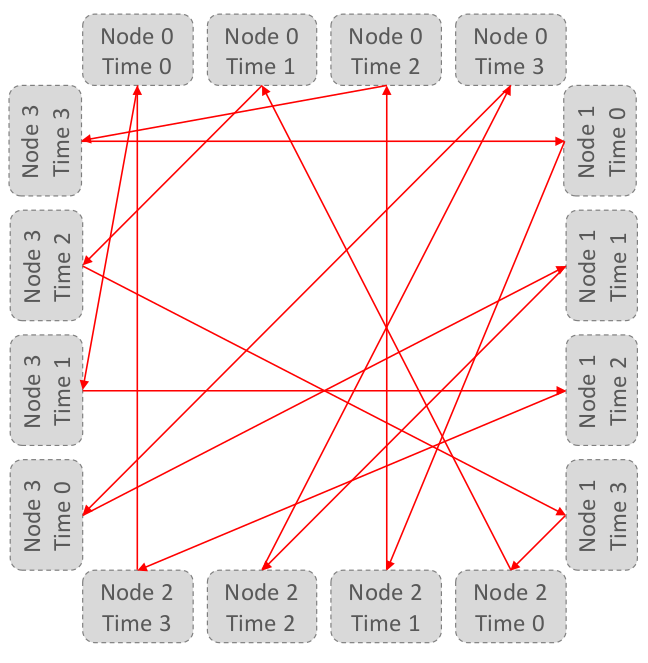
\includegraphics[scale=0.2]{figures/salesman-penalties7.png} &
			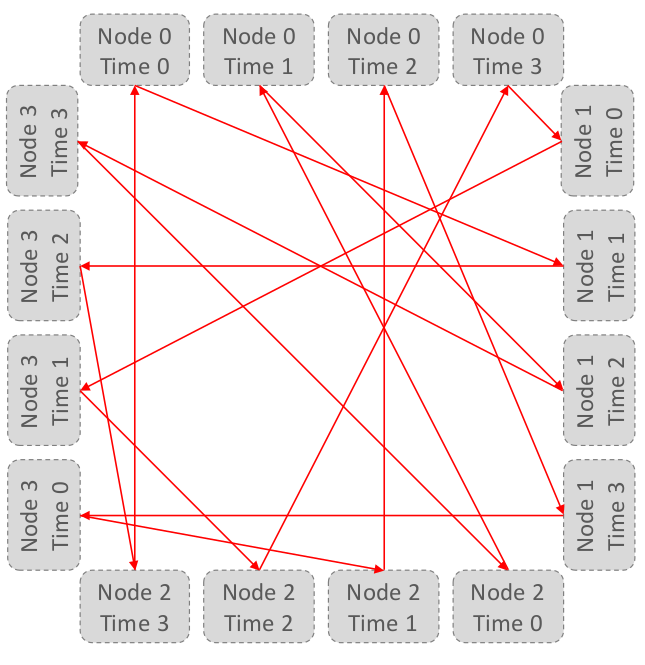
\includegraphics[scale=0.2]{figures/salesman-penalties8.png} &
			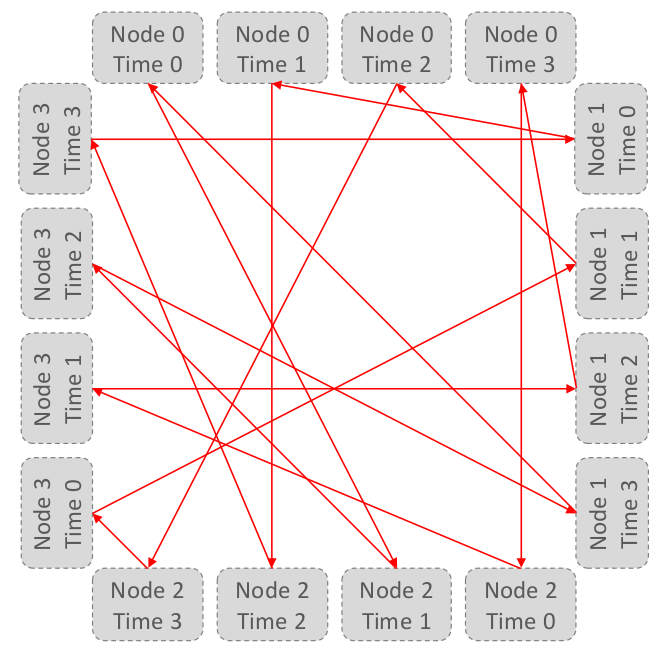
\includegraphics[scale=0.2]{figures/salesman-penalties9.png} \\
			
			7: Type D tours & 8: Type E tours & 9: Type F tours \\
		\end{tabular}
	}
	\caption{Representación gráfica de las penalizaciones entre las distintas intereracciones}
	\label{fig:salesman-penalties}
\end{table}

\subsection{El ensamblaje del genoma}

El genoma de un organismo contiene toda su información genética. Dicha información se almacena en el ADN (o en el ARN para ciertos organismos) como cadenas de nucleótidos de entre las cuatro siguientes:

\begin{itemize}
	\item Adenina (A)
	\item Timina (T)
	\item Citosina (C) 
	\item Guanina (G)
\end{itemize}

Los nucleótidos se colocan en parejas (llamadas \emph{base-pairs} o simplemente bp) en un doble hélice que contiene la información duplicada. Es decir, esta codificación de la información se traduce en una secuencia de letras entre las cuatro posibilidades anteriores. Sin embargo, los dispositivos actuales permiten leer unicamente hasta $1000$ bp, teniendo el ADN humano aproximádamente 3 Mbp. \\

\textbf{El problema del ensamblaje del genoma} consiste en, a partir de un gran conjunto de pequeñas lecturas, recomponer la cadena de ADN original de la que provienen estas lecturas. \\

Cabe destacar que nos centramos el método denominado \emph{de novo} que no utiliza referencia conocida sobre el ADN de la especie, como si hace el método \emph{ab initio}, añadiendo sesgo. De la misma forma, todo este proceso es equivalente para el ARN aunque las parejas de nucleótidos que lo componen son distintas. \\

El procedicimiento seguido es transformar este problema en el problema del viajante de comercio, que ya sabemos imbuir en nuestras arquitecturas D-Wave, para posteriormente resolverlo utilizando \emph{quantum annealing}. Para ello creamos un grafo donde cada nodo tiene asignada una cadena. Asignamos pesos a los lados del grafo según lo bien que se solapen dichas cadenas de nucleótidos. Un camino hamiltoniano en este grafo será una ordenación de las cadenas. Si minimizamos los pesos de dicho camino hamiltoniano obtenemos la ordenación que maximiza el pegado entre cadenas. Esto es, la ordenación que recompone el ADN original. A este grafo se le denomina \textbf{grafo Overlap-Layout Consensus (OLC)}.\\

\begin{figure}[H]
	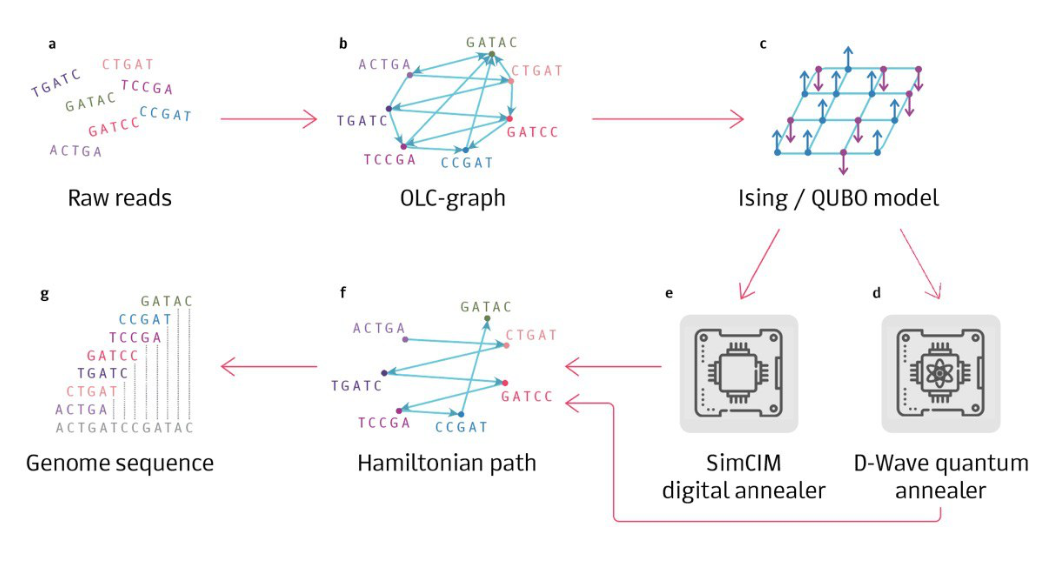
\includegraphics[scale=0.4]{figures/de-novo-process.png}
	\centering
	\caption{Diagrama del proceso de resolución del ensamblaje del genoma utilizando quantum annealing}
\end{figure}

\subsection{Resultados experimentales}

Comentaremos unicamente algunos de los experimentos llevados acabo utilizando los computadores D-Wave. En primer lugar, considerémos un ejemplo con únicamente 4 lecturas:

\begin{itemize}
	\item $r0 = ATGGCGTGCA$
	\item $r1 = GCGTGCAATG$
	\item $r2 = TGCAATGGCG$
	\item $r3 = AATGGCGTGC$
\end{itemize}

Donde la solución es unir las lecturas en orden alfanumérico: $r0 \rightarrow r1 \rightarrow r2 \rightarrow r3$. El grafo OLC asociado a este problema es justamente el de la figura \ref{fig:salesman-example}. Estudiando este gráfico nos damos cuenta de que hay 6 tipos de ciclo en el mismo, plasmados en la sigueinte figura:

\begin{table}[H]
	\centering
	\begin{tabular}{ccc}		
		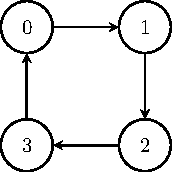
\includegraphics[scale=.9]{figues/salesman-cycleA.pdf} &
		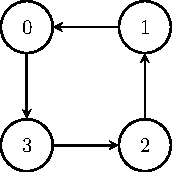
\includegraphics[scale=.9]{figues/salesman-cycleB.pdf} &
		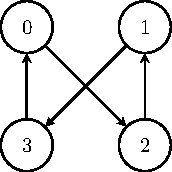
\includegraphics[scale=.9]{figues/salesman-cycleC.pdf} \\
		
		Tipo A & Tipo B & Tipo C \\
		
		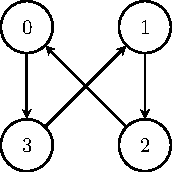
\includegraphics[scale=.9]{figues/salesman-cycleD.pdf} &
		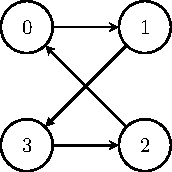
\includegraphics[scale=.9]{figues/salesman-cycleE.pdf} &
		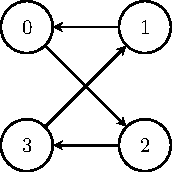
\includegraphics[scale=.9]{figues/salesman-cycleF.pdf} \\
		
		Tipo D & Tipo E & Tipo F \\
	\end{tabular}
	\caption{Tipos de ciclos de un grafo de $4$ nodos}
	\label{tbl:salesman-cycles}
\end{table}

Analizando estos ciclos podemos darnos cuenta de que el tipo de ciclo con menor longitud de pegado (también denominada energía) es el tipo A, como cabría esperar pues esta es la solución. Además, los tipos C, D, E y F tienen todos la misma energía. En último lugar, el ciclo de tipo B tiene la mayor energía de todas.

\begin{figure}[H]
	\makebox[\textwidth][c]{
		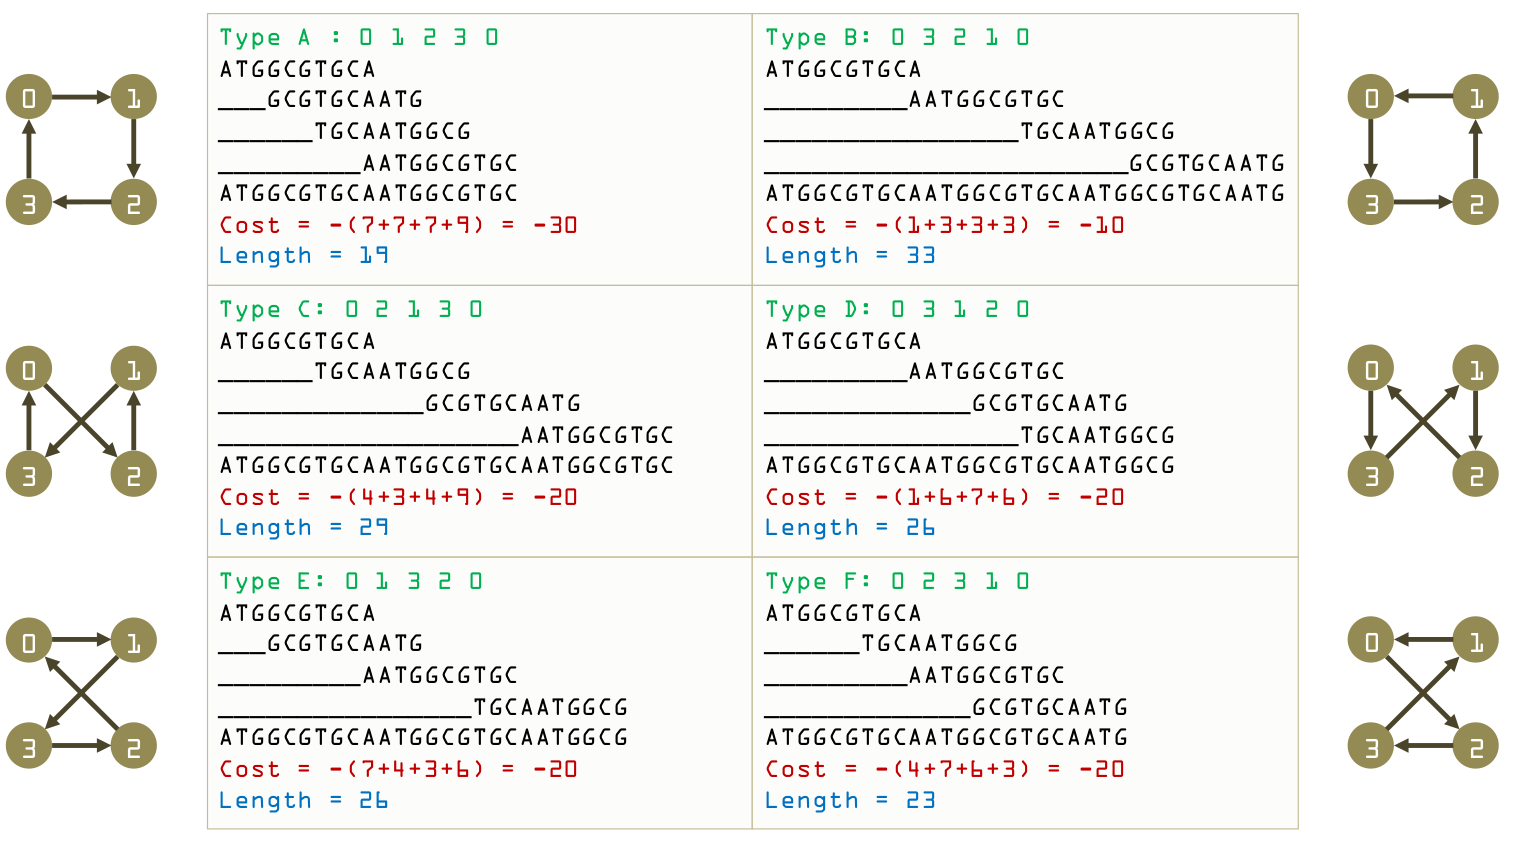
\includegraphics[scale=0.35]{figues/overlap-cycles.png}
	}
	\centering
	\caption{Energía y pegado de los distintos tipos de ciclos.}
\end{figure}

En primer lugar, utilizamos un Simulated Annealer, también de la empresa D-Wave, para resolver este problema. Para ello basta con configurar correctamente la matriz Q asociada al problema y conectarse a la API de D-Wave para transmitir esta información. Obtenemos los siguientes resultados:

\begin{table}[H]
	\centering
	\begin{tabular}{lrr}
		\textbf{Tipo de ciclo} & \textbf{Ocurrencias} & \textbf{Energía} \\
		\hline
		Tipo A	& 3722	& -7.9811	\\
		Tipo C	& 1474	& -7.4541	\\
		Tipo D	& 1469	& -7.4541	\\
		Tipo F	& 1458	& -7.4541	\\
		Tipo E	& 1431	& -7.4541	\\
		Tipo B	& 446	& -6.927                             
	\end{tabular}
	\caption{Results of experiment 2}
	\label{tab:exp2}
\end{table}

\begin{figure}[H]
	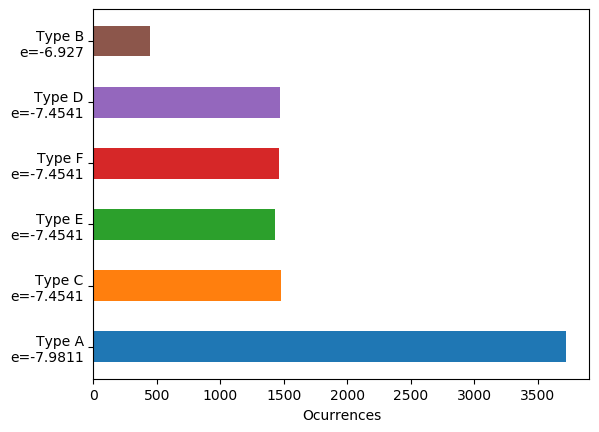
\includegraphics[scale=0.8]{figures/experiment2.png}
	\centering
	\caption{Ocurrencias de cada tipo de ciclo utilizando Simulated Annealing en $10.000$ realizaciones.}
	\label{fig:exp2-occ}
\end{figure}

Realizamos el mismo experimento $10.000$ veces y obtenemos la distribución de la figura \ref{fig:exp2-occ}. Estos resultados encajan por completo con el análisis teórico realizado, pues el tipo más frecuente es el A, solución de nuestro problema. Los tipos C, D, E y F obtienen aproximadamente el mismo número de ocurrencias pues tenían la misma energía. Finalmente, el tipo B es el menos común. \\

Repetimos el experimento utilizando el ordenador cuántico D-Wave 2000. Para ello damos distintos valores a los parámetros. En particular, fijamos $a=-X$ y $b=c=X$ para distintos valores de $X$. Los mejores resultados se obtuvieron para $X = 1.5$ y $1.6$, y se muestran a continuación:

\begin{table}[H]
	\centering
	\begin{tabular}{lrrr}
		\textbf{Tipo de ciclo} & \textbf{Ocurrencias (X=1.5)} & \textbf{Ocurrencias (X=1.6)} & \textbf{Energía} \\
		\hline
		Tipo A	& 131	& 50	& -7.9811	\\
		Tipo C	& 124	& 46	& -7.4541	\\
		Tipo D	& 40	& 91	& -7.4541	\\
		Tipo F	& 55	& 117	& -7.4541	\\
		Tipo E	& 112	& 118	& -7.4541	\\
		Tipo B	& 99	& 64	& -7.4541	\\    
		Inválidos & 9221	& 9194	& $>$ -5.6433                         
	\end{tabular}
	\caption{$10.000$ ocurrencias utilizando D-Wave 2000Q.}
	\label{tab:exp3}
\end{table}

\begin{figure}[H]
	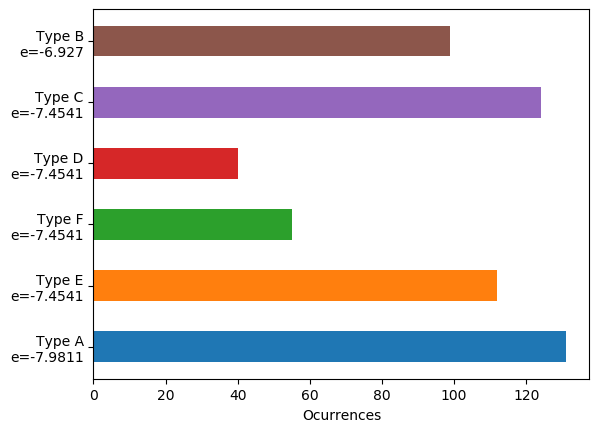
\includegraphics[scale=0.75]{figures/experiment3 (1.5).png}
	\centering
	\caption{Ocurrences of each cycle type in a $10.000$ reads experiment using Quantum Annealing, filtering out invalid cycles, with QUBO parameters $(-1.5; 1.5; 1.5)$}
	\label{fig:exp3-occ1}
\end{figure}

\begin{figure}[H]
	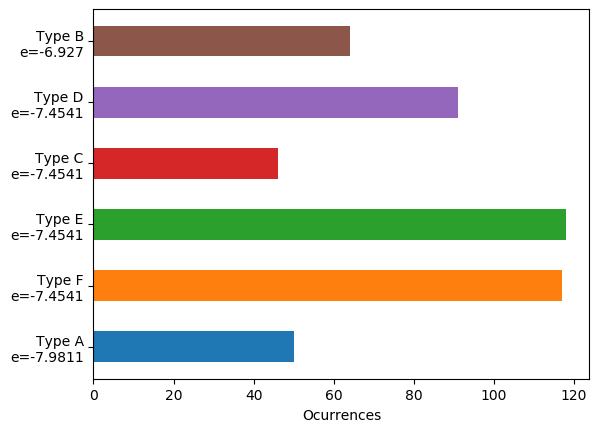
\includegraphics[scale=0.75]{figures/experiment3 (1.6).png}
	\centering
	\caption{Ocurrences of each cycle type in a $10.000$ reads experiment using Quantum Annealing, filtering out invalid cycles, with QUBO parameters $(-1.6; 1.6; 1.6)$}
	\label{fig:exp3-occ2}
\end{figure}


\section{Conclusiones}

\end{document}
